\chapter{Dodatek}
\label{dodatek}

\section{Instalace pluginu}

Popis instalace pluginu je uveden pro software QGIS nastavený v anglickém jazyce. 

\subsection{Instalace pluginu pomocí QGIS repozitáře}

Pro nainstalování pluginu \textit{GTFS Loader} v softwaru QGIS se nejprve vybere přes menu 
panel \textit{Plugins} a poté z nabídky panelu se vybere možnost \textit{Manage and Install Plugins...}.
Dále se otevře dialogové okno pro výběr instalace pluginu z QGIS repozitáře, zadá se název
plugin a stiskne se tlačítko \textit{Install Plugin}.

V QGIS repozitáři je aktuálně uložena verze plugine 1.0, která nedisponuje vytvářením
tarifních pásem.  

\begin{figure}[H] \centering
    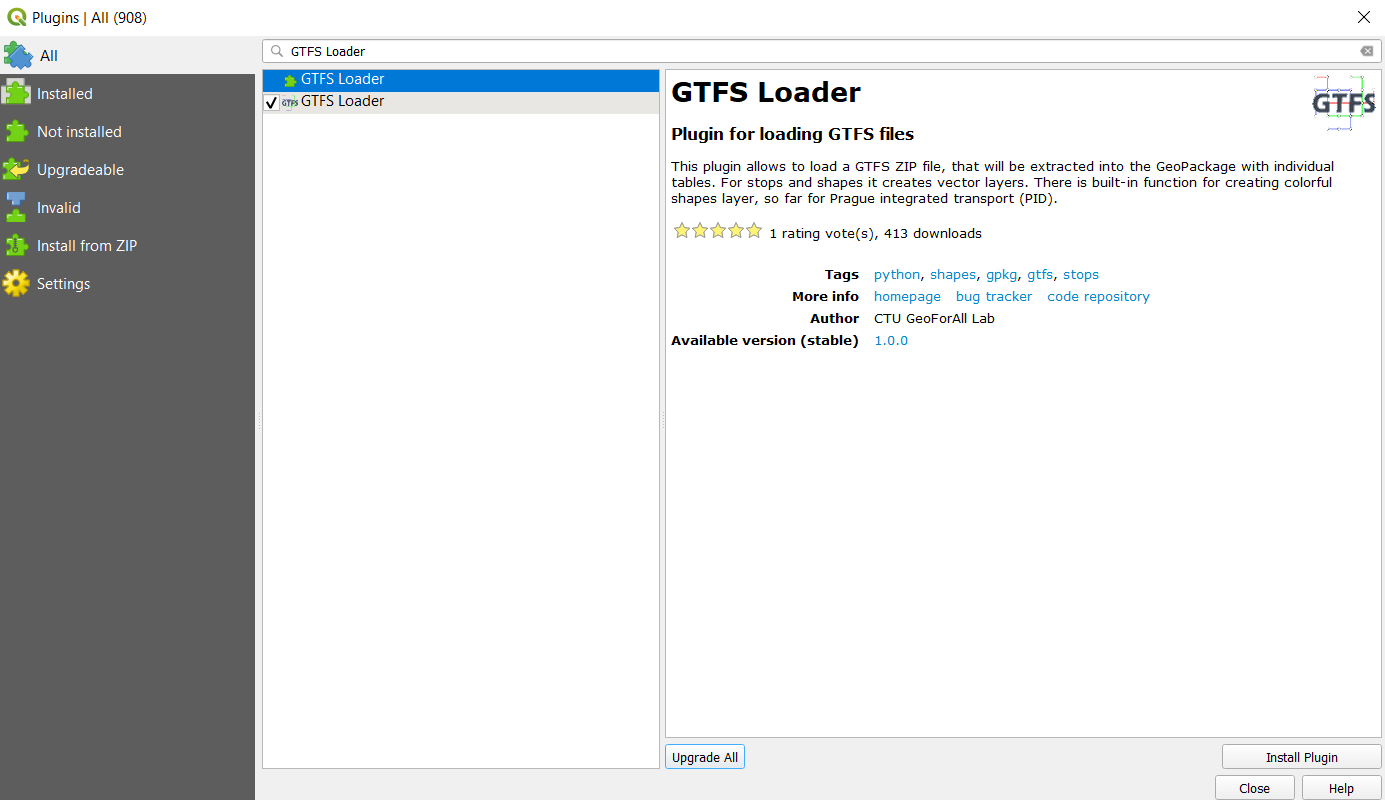
\includegraphics[width=400pt]{./pictures-dodatek/repositary.png}
    \caption[Dialogové okno pro výběr instalace pluginu z QGIS repozitáře]{Dialogové okno pro výběr instalace pluginu z QGIS repozitáře}
	\label{fig:repositary}              
\end{figure} 

\subsection{Instalace pluginu pomocí ZIP souboru}

K nainstalování experimentální verze pluginu 2.0 je třeba zvolit jiný postup.
Z uvedeného odkazu \href{https://github.com/ctu-geoforall-lab/qgis-gtfs-plugin/tree/pid\_zones}
{https://github.com/ctu-geoforall-lab/qgis-gtfs-plugin/tree/pid\_zones}, který směřuje na repozitář
pluginu \textit{GTFS Loader} ve službě GitHub, je potřeba stáhnout komprimovaný \zk{ZIP} soubor. 
To se provede tak, že se rozklikne tlačítko \textit{Code} a následně se vybere možnost
\textit{Download ZIP}.  

Pro načtení \zk{ZIP} souboru v softwaru QGIS je potřeba otevřít stejné dialogové okno,
jako při instalaci pomocí QGIS repozitáře, ale následně se vybere možnost \textit{Install from ZIP}. 
Do uvedeného pole se zadá celá cesta ke staženému \zk{ZIP} souboru a poté se stiskne tlačítko
\textit{Install Plugin}.

\begin{figure}[H] \centering
    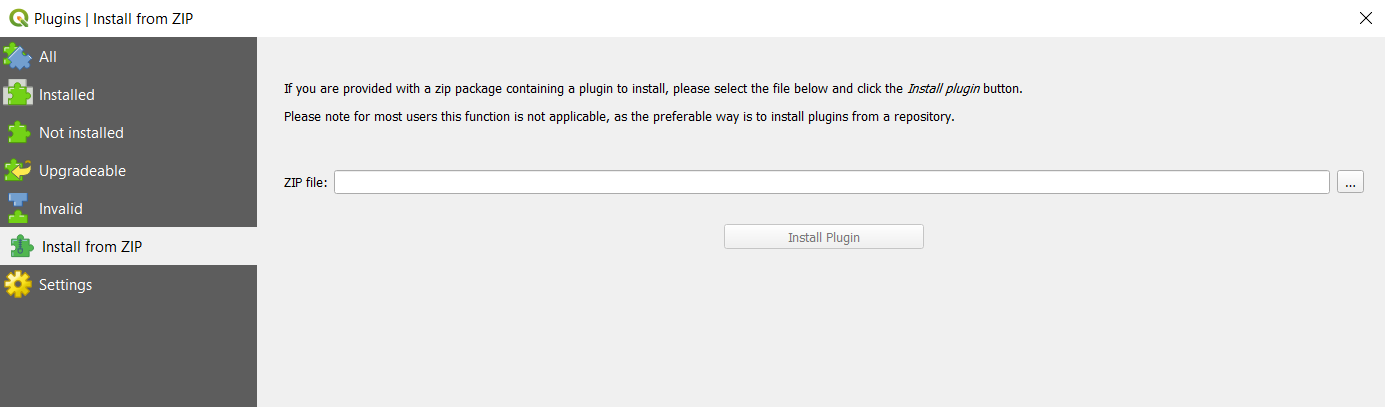
\includegraphics[width=400pt]{./pictures-dodatek/zip.png}
    \caption[Dialogové okno pro výběr \zk{ZIP} souboru]{Dialogové okno pro výběr \zk{ZIP} souboru}
	\label{fig:zip}              
\end{figure} 

\section{Použití pluginu pro vytvoření tarifních pásem}

Po instalaci se objeví plugin \textit{GTFS Loader} v panelu \textit{Plugins} anebo jako ikona pluginu
v panelu nástrojů. Po stisknutí ikony se v levém dolním rohu objeví dialogové okno pluginu.

\begin{figure}[H] \centering
    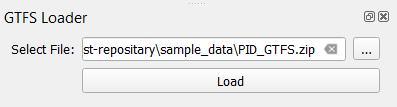
\includegraphics[width=200pt]{./pictures-dodatek/plugin.png}
    \caption[Dialogové okno pluginu GTFS Loader]{Dialogové okno pluginu GTFS Loader}
	\label{fig:gtfs_loader}              
\end{figure} 

Do pole s popiskem \textit{Select File} se musí vyplnit kompletní cesta k GTFS \zk{ZIP} souboru (
pro vytváření pásem pouze k PID\_GTFS \zk{ZIP} souboru). Dále stačí stisknout tlačítko \textit{Load}.
Následně se zobrazí další dialogové okno, zda uživatel chce vytvořit tarifní pásma. Stiskne se
\textit{Yes} a proces plugin již běží na pozadí. Délka času tvorby závisí na výkonu počítače. 
Během procesu uživatel vidí informace o progresu v ukazateli průběhu (ProgressBar). 

Po načtení dat se v mapovém okně zobrazí kromě vrstvy \textit{shapes} a \textit{stops} i vrstva 
\textit{zones}. Na obrázku \ref{fig:gtfs_loader_vysledek} je vrstva \textit{zones}
jako nejníže položená. Tyto vrstvy jsou se stejným názvem uloženy i v seznamu vrstev ve skupinách.

\begin{figure}[H] \centering
    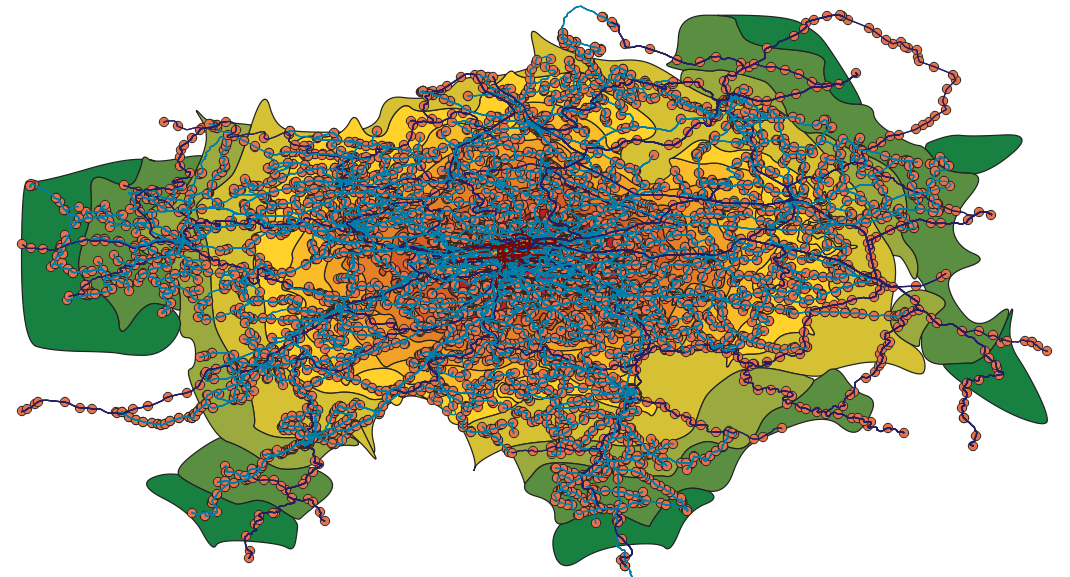
\includegraphics[width=400pt]{./pictures-dodatek/visualization.png}
    \caption[Výsledek procesu pluginu]{Výsledek procesu pluginu}
	\label{fig:gtfs_loader_vysledek}              
\end{figure} 